\documentclass[11pt,aspectratio=1610,dvipsnames]{beamer}
\graphicspath{{figs/}}
\usetheme{default}
\usepackage{DasBeamerPaket}
\usepackage{animate}
\usepackage{lastpage}
\usepackage{tikz}
\setbeamercolor{section in toc}{fg=NavyBlue}
\setbeamercolor{frametitle}{fg=NavyBlue}
\captionsetup[figure]{labelfont=bf}
\captionsetup[table]{labelfont=bf}
\setbeamertemplate{caption}[numbered]
\newcommand{\btheta}{\boldsymbol{\theta}}
\begin{document}

	\title{Event Selection for $\eta'$ analysis}
	\subtitle{Analysis Meeting}
	\definecolor{myWhite}{rgb}{1,1,1}
	
	\setbeamertemplate{footline}[text line]{\parbox{0.3\linewidth}{\vspace*{-9pt}\textcolor{white} \insertsection  \hfill} \parbox{0.7\linewidth}{\vspace*{-8pt} \textcolor{white}{\hfill\hspace{-3cm}\insertshorttitle \phantom{ }-- \insertshortsubtitle}  \hfill \textcolor{myWhite}{\insertpagenumber/\pageref{LastPage}}}}
	
	\addtobeamertemplate{footline}{ \makebox[0pt][l]{\hspace{-1cm}
			\raisebox{0cm}[0pt][0pt]{\colorbox{gray!15!black}{\phantom{{\large TEXTTEXTTEXTTEXTTEXTTEXTTEXTTEXTTEXTTEXTTEXTTEXTTEXTTEXTTEXTTEXTTEXTTEXTTEXTTEXTTEXTTEXTTEXTTEXTTEXTTEXTTEXTTEXTTEXTTEXTTEXTTEXTTEXTTEXTTEXTTEXTTEXTTEXTTEXTTEXT}}}}}}
	
	\setbeamercovered{transparent}
	\setbeamertemplate{navigation symbols}{}
	\setbeamertemplate{frametitle}[default][left,leftskip=0.5cm]
	%
	\setbeamertemplate{itemize item}{\color{black}$\blacktriangleright$}
	\setbeamertemplate{section in toc}[sections numbered]
	\captionsetup{font=scriptsize,labelfont=scriptsize}
	
	\AtBeginSection[]
	{	
		\definecolor{myWhite}{rgb}{0,0,0}
		\begin{frame}[noframenumbering]
			\frametitle{}
			\addtocounter{page}{-1}
			\tableofcontents[currentsection]
			
		\end{frame}
		\definecolor{myWhite}{rgb}{1,1,1}
	}
	
\begin{frame}{Event selection for $\eta'$ analysis }
	$\eta'\to\gamma\gamma$: 2PED and 3PED with charge information (12/2017, 05/2018 beamtime):
	\begin{figure}
		\centering
			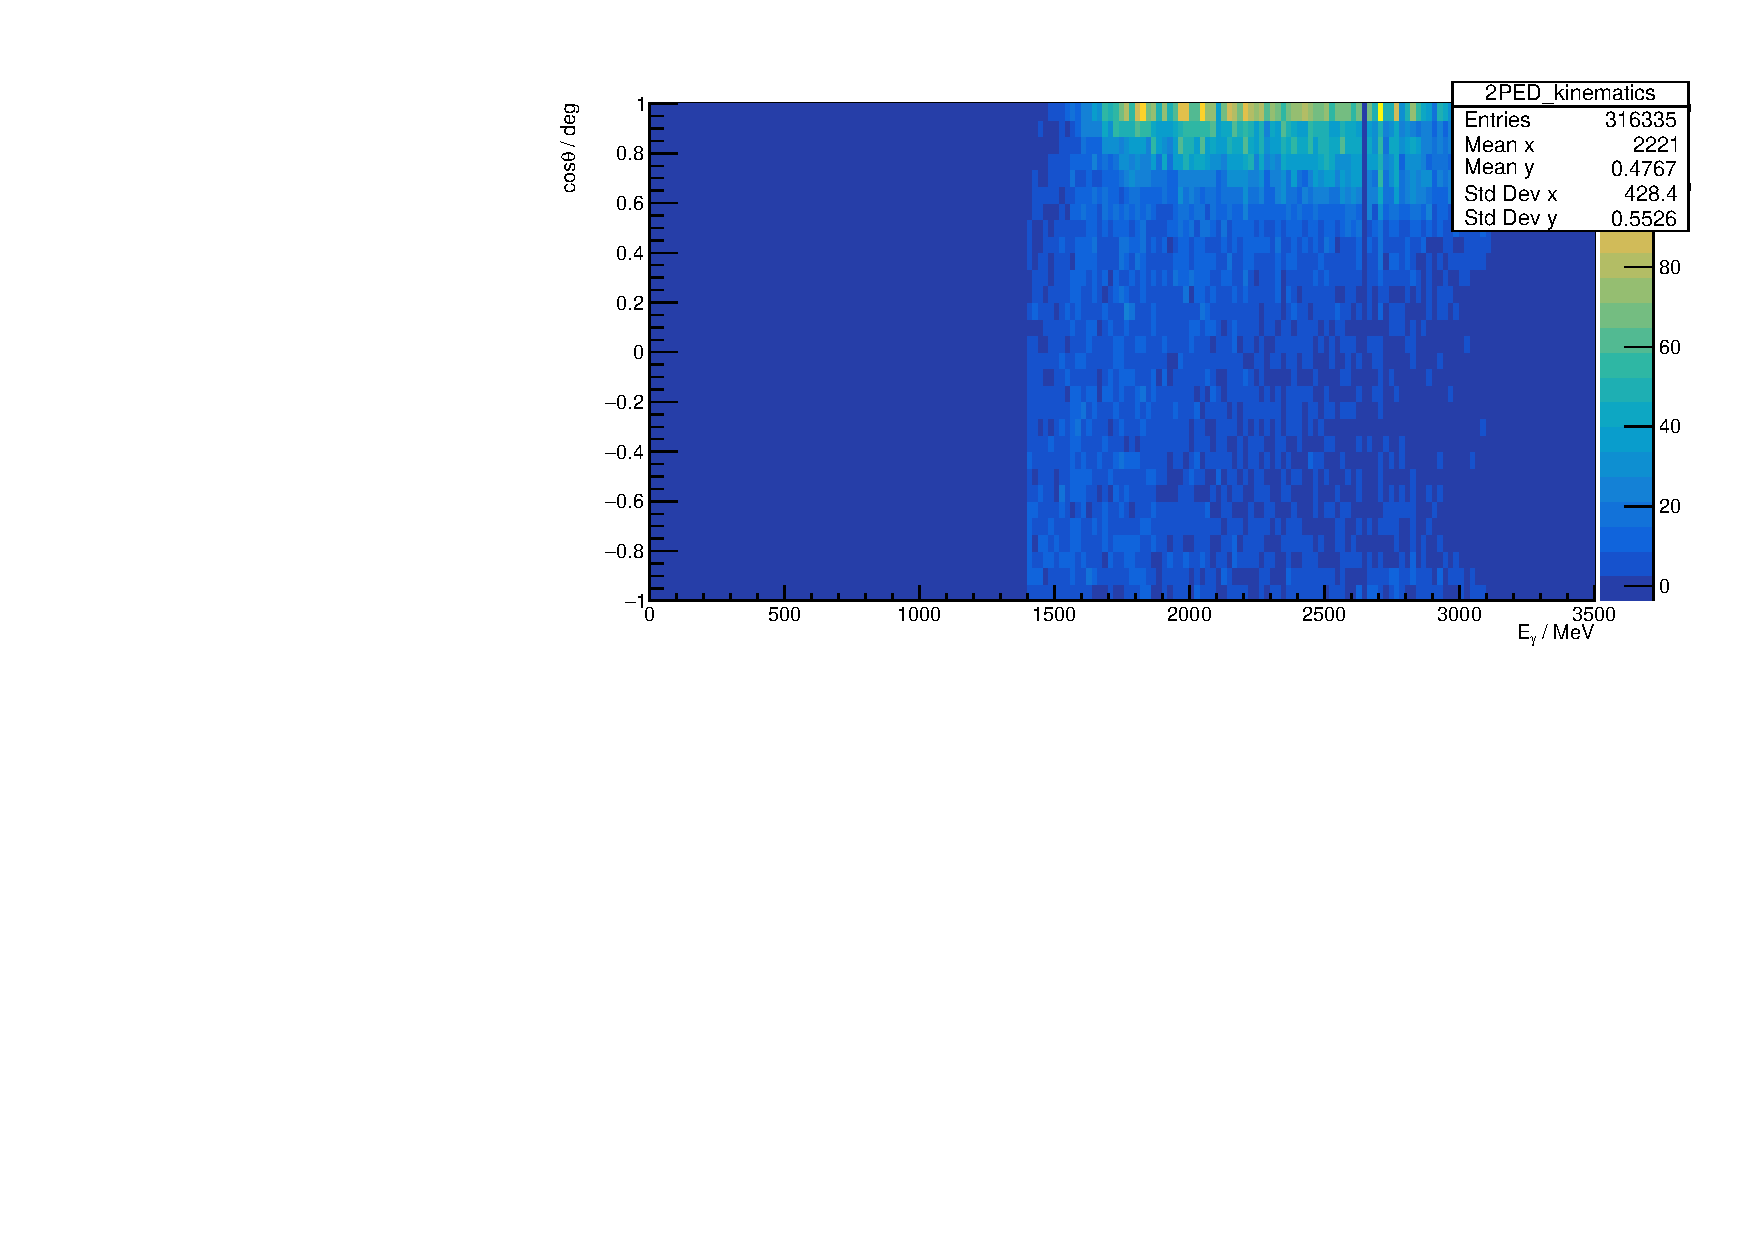
\includegraphics[width=.49\linewidth]{../../figs/2PEDs.pdf}
		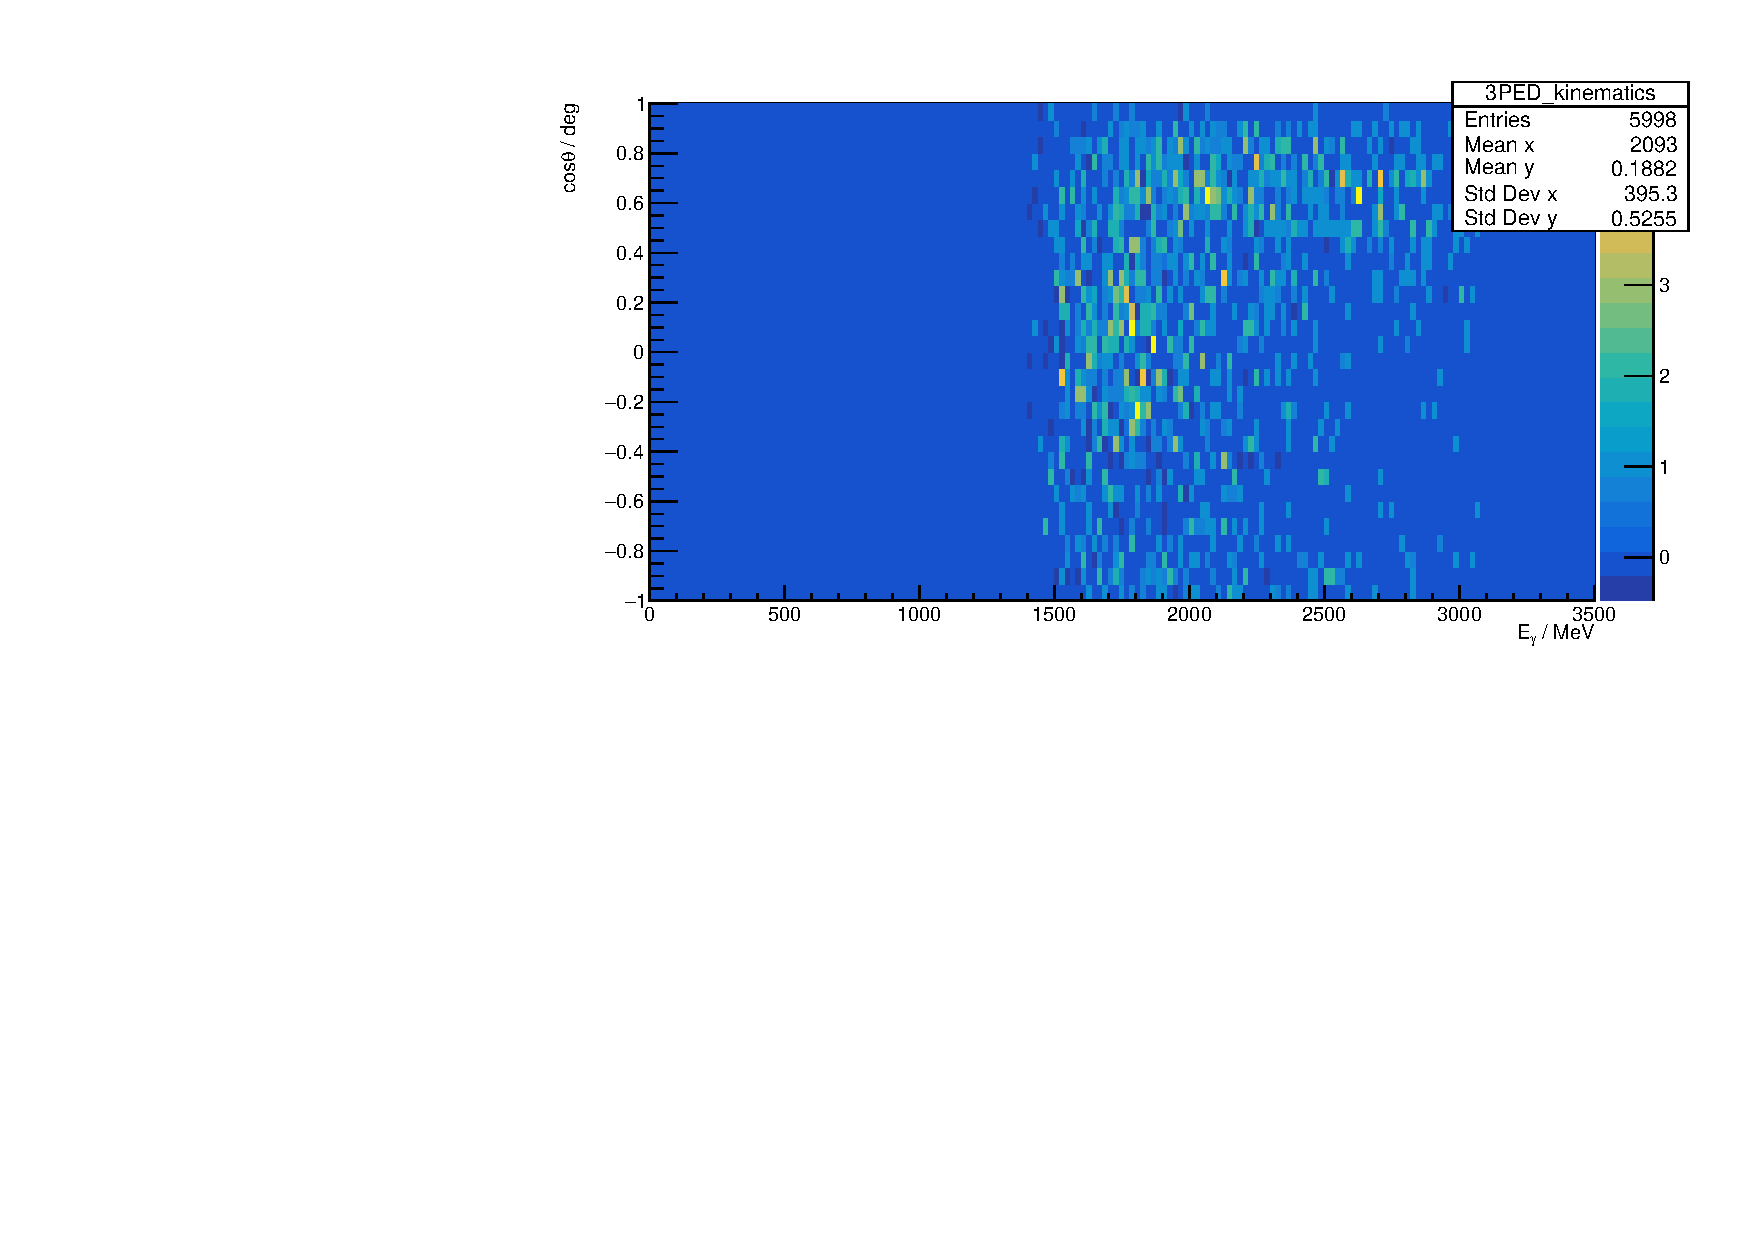
\includegraphics[width=.49\linewidth]{../../figs/3PEDs.pdf}
	\end{figure}
\begin{itemize}
 	\item 2PEDs are mostly very forward events  and mostly carbon 
 	\item keep the few 3PEDs
\end{itemize}
\end{frame}	
\begin{frame}{}
employ cuts on reaction time and meson-proton-time...
	\begin{figure}
		\centering
		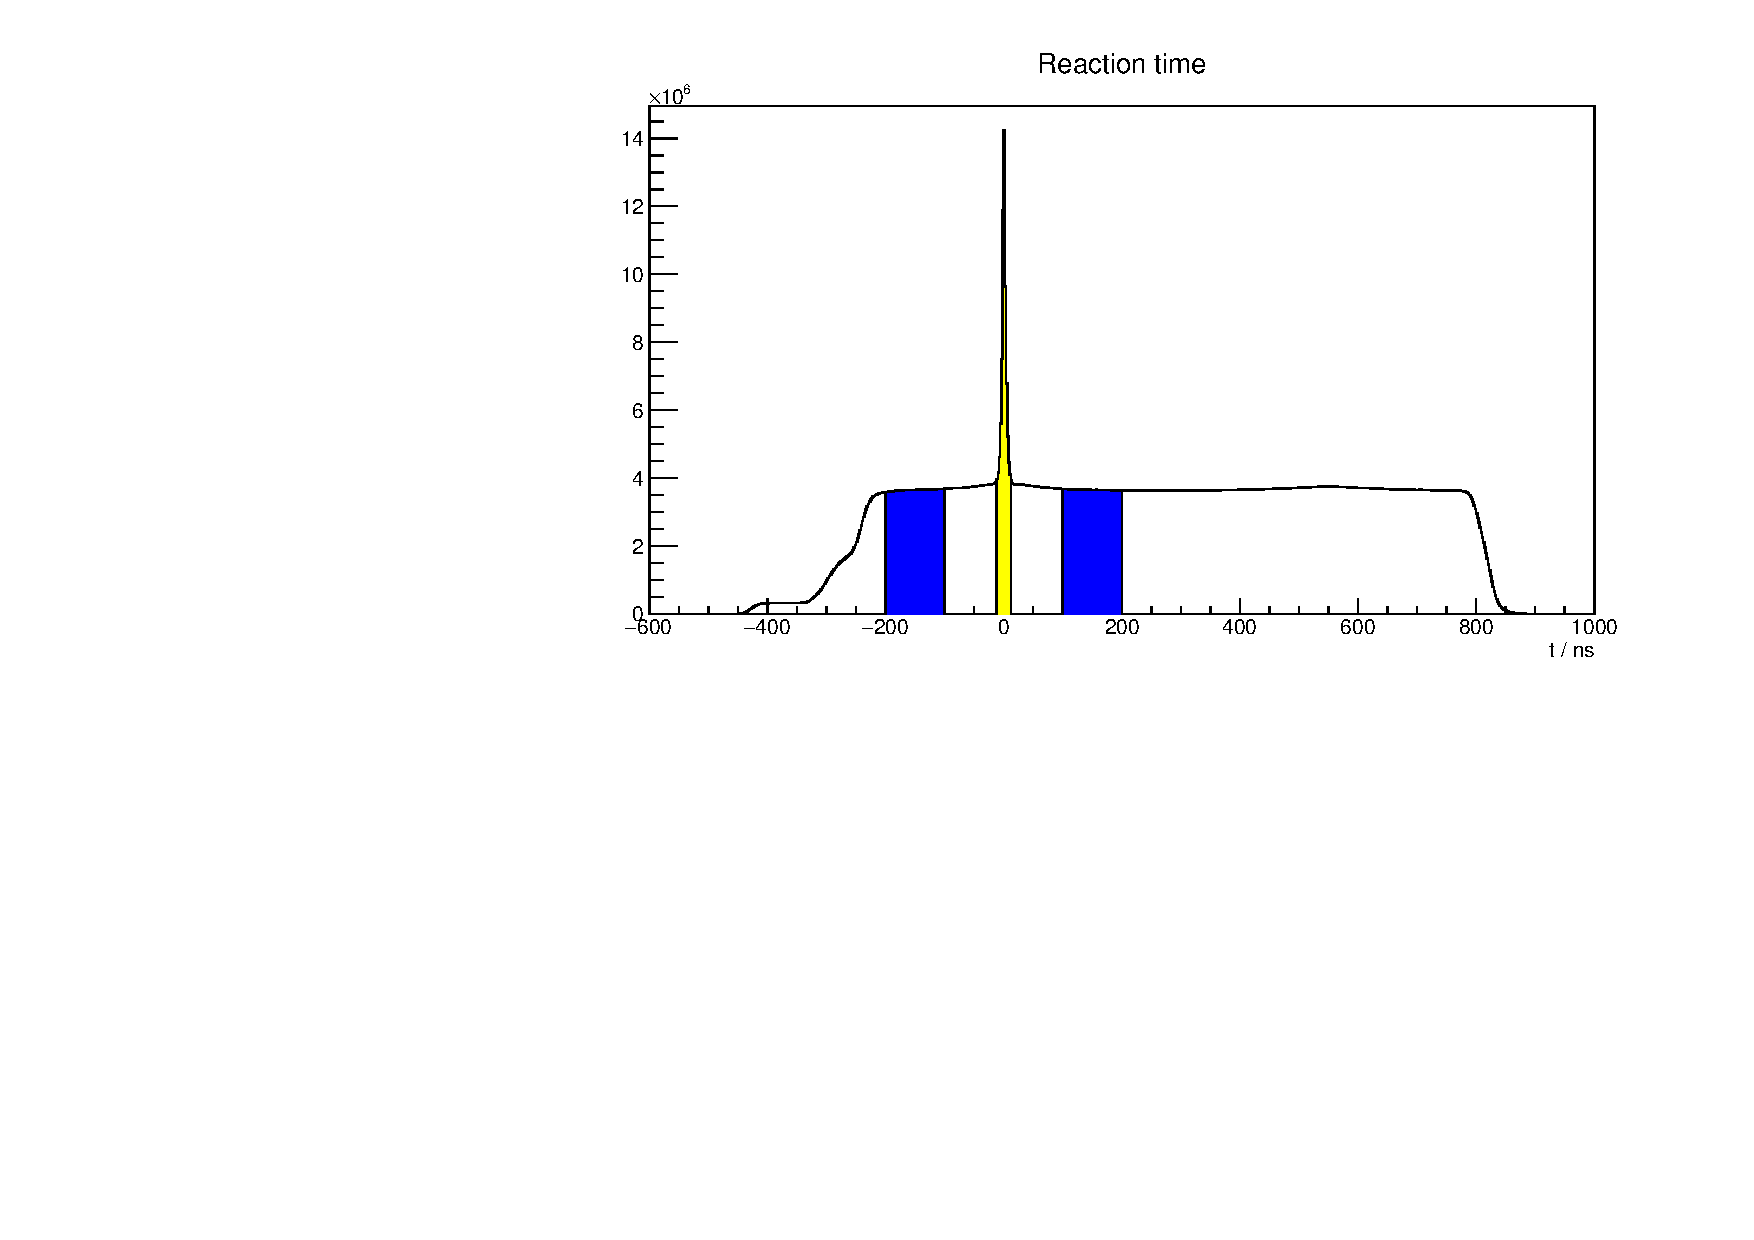
\includegraphics[width=.49\linewidth]{../../figs/reaction_time_cut.pdf}
		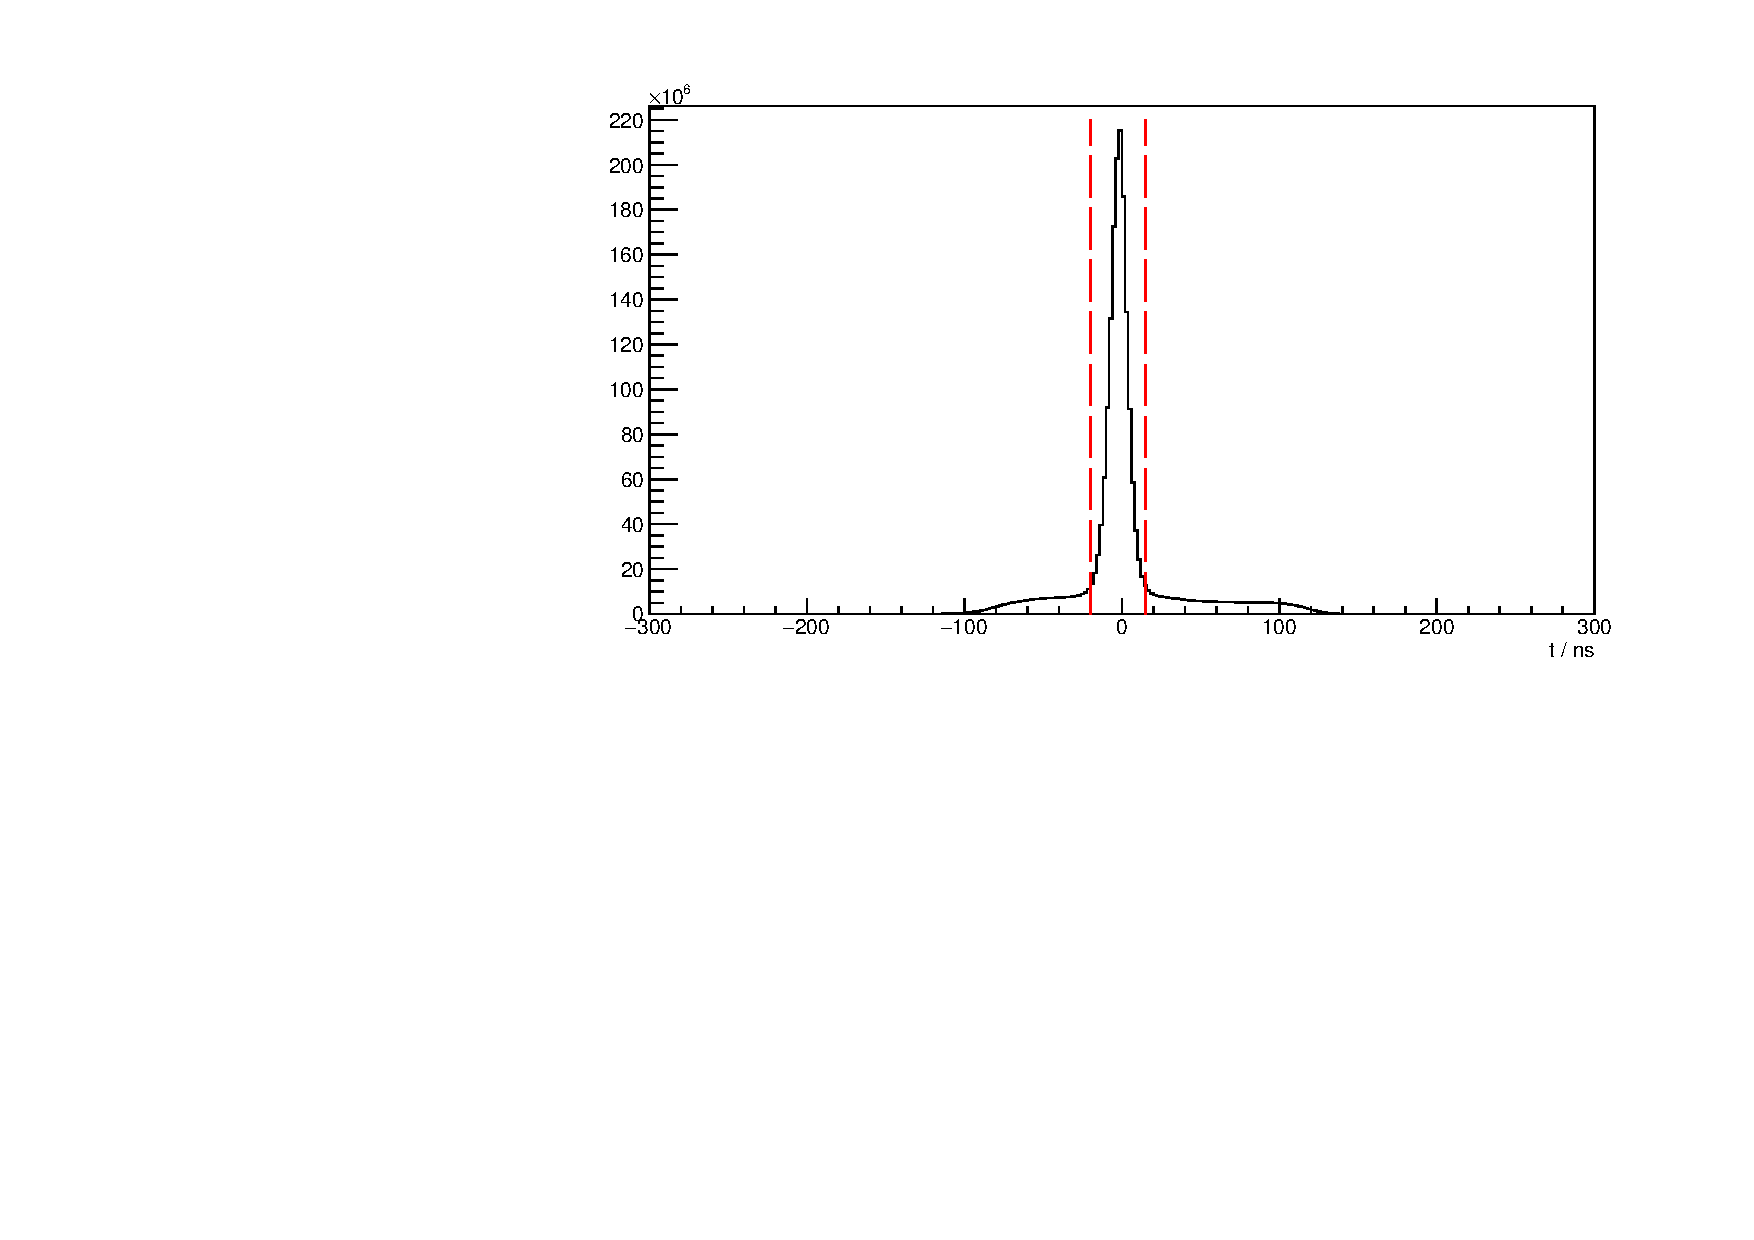
\includegraphics[width=.49\linewidth]{../../figs/meson_time_cut.pdf}
	\end{figure}
\end{frame}	
\begin{frame}{}
...and the usual kinematic cuts (carbon from 05/2018, in addition: $E_\gamma>\SI{1400}{\mega\eV}$)
	\begin{figure}
		\centering
		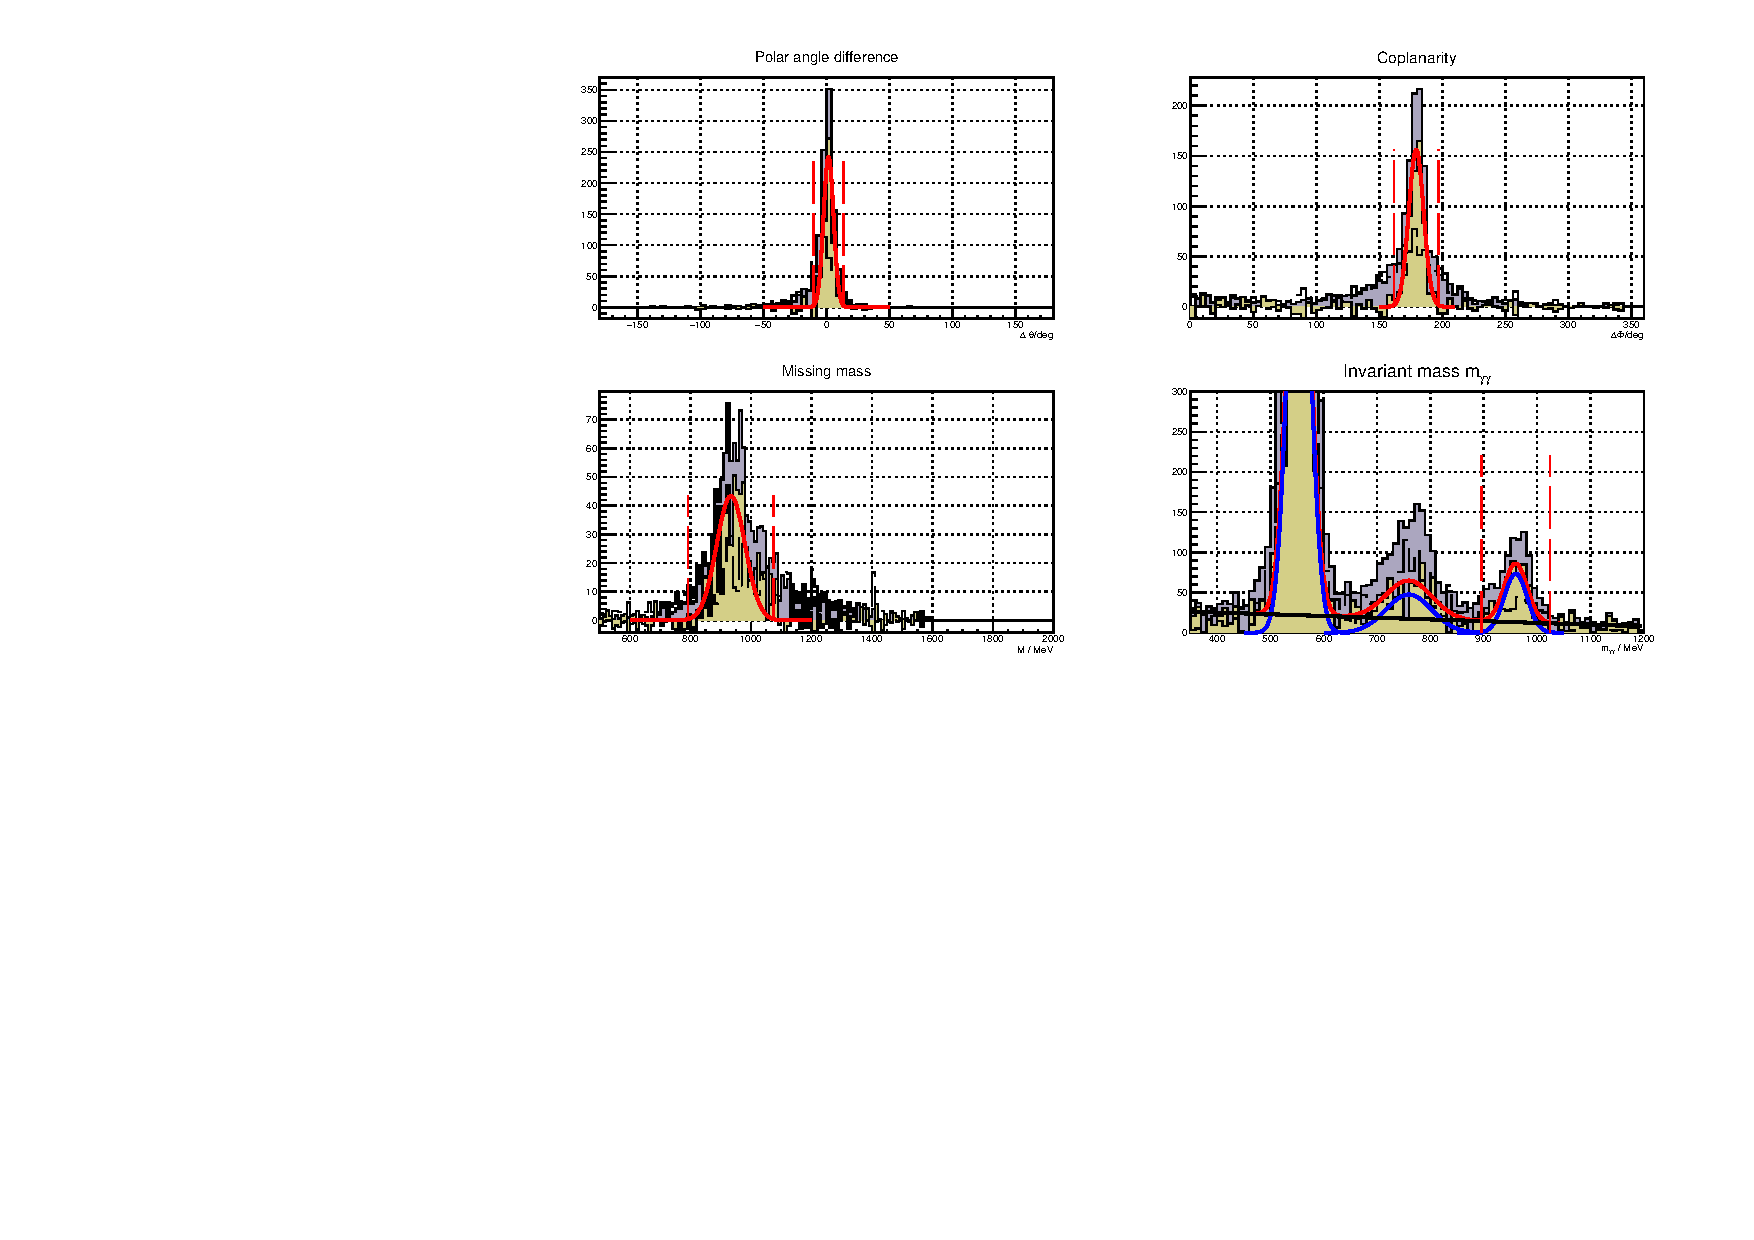
\includegraphics[width=\linewidth]{../../figs/cuts.pdf}
	\end{figure}
\end{frame}	
\begin{frame}{}
total yield:
	\begin{figure}
		\centering
		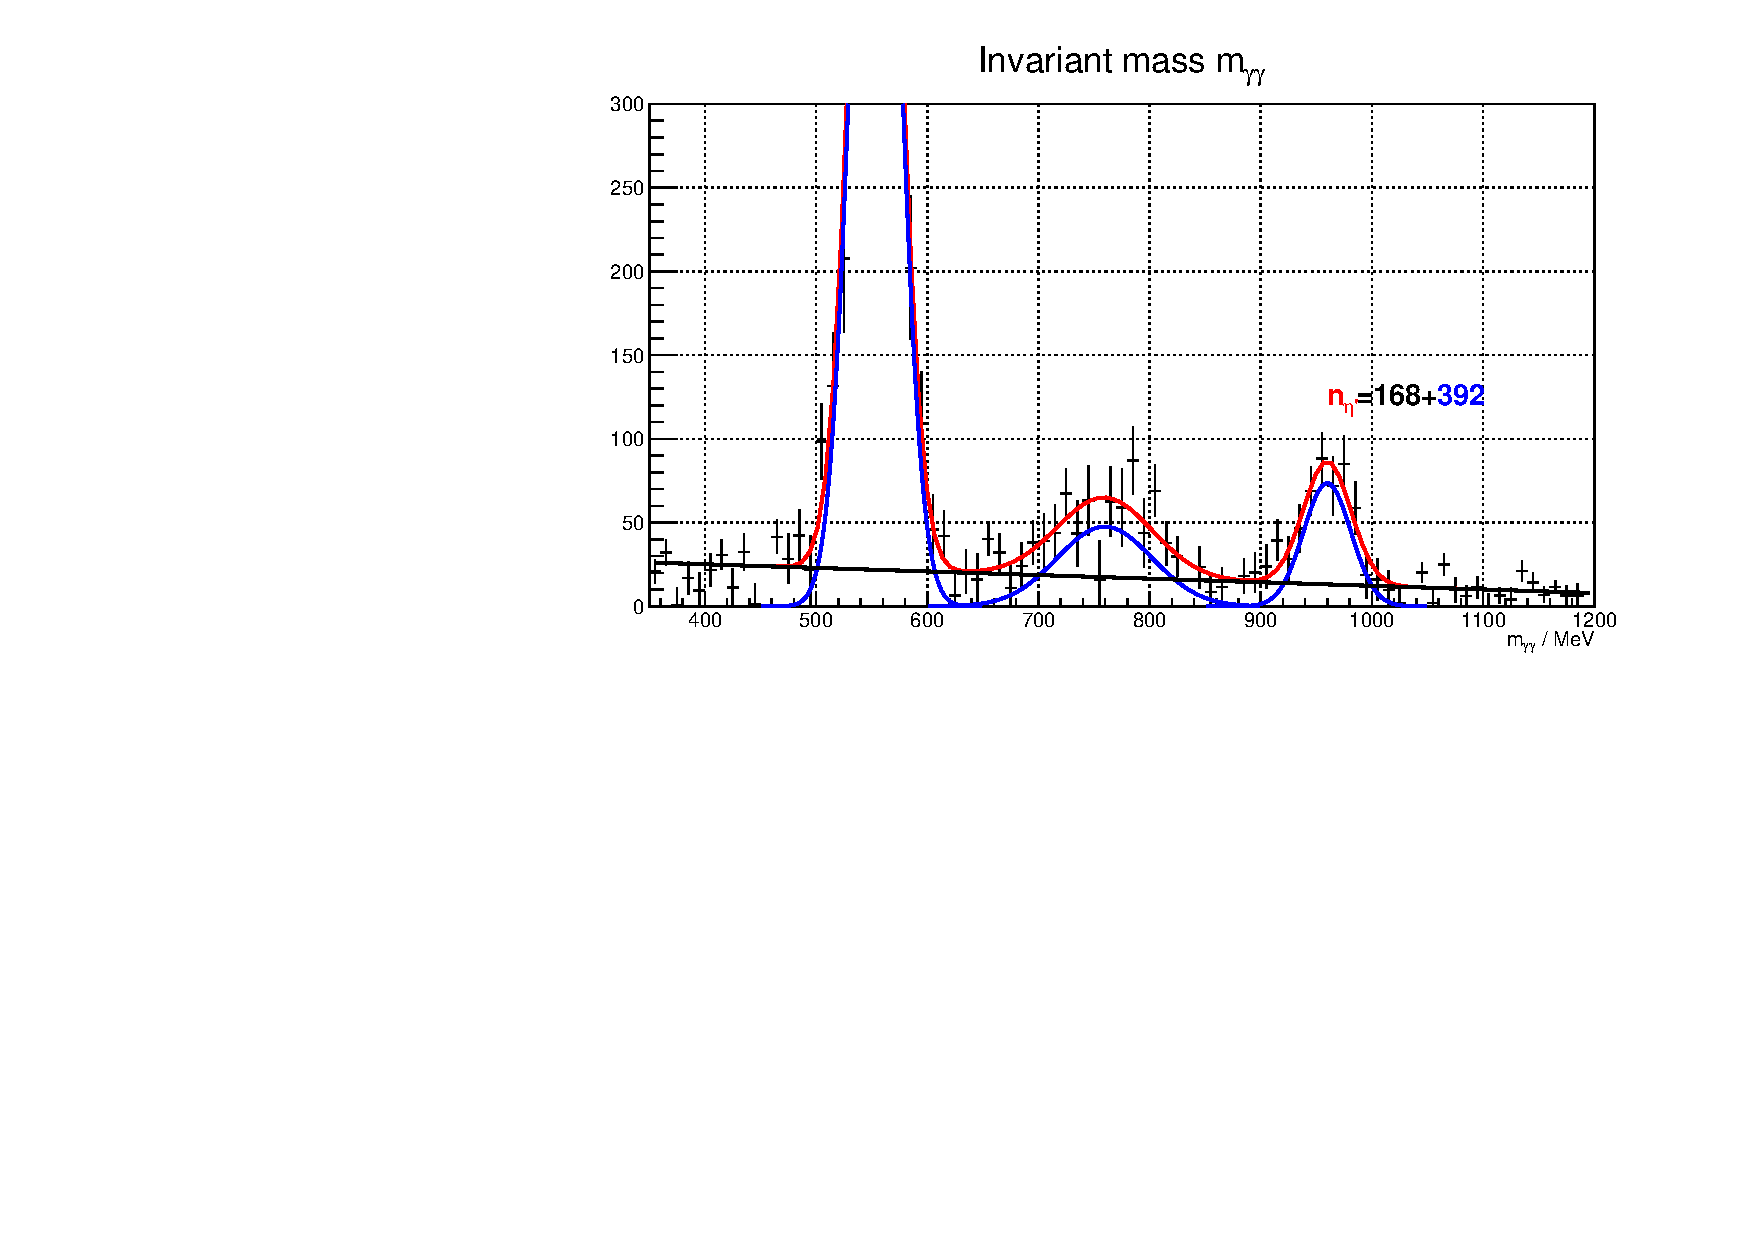
\includegraphics[width=\linewidth]{../../figs/etap_yield_total.pdf}
	\end{figure}
TBD: background in missing mass spectrum, inv. mass spectrum, with MC
\end{frame}	
\end{document}